\section{随机Top-$k$算法}
\label{sec:randomized_topk:method}
本章节将提出随机Top-$k$算法,其优势来自于两个方面:
(1)从模型泛化(Generalization)角度,Top-$k$稀疏化优于缩小拆分层,因为同等压缩比率下,Top-$k$稀疏化能够提供更大的表征空间和决策边界大小。
(2)从模型训练和收敛的角度,Top-$k$会导致部分神经元训练困难,导致收敛变慢,并且无法完全利用表征空间,从而降低其泛化性能上的优势。
%
基于以上两个观察,我们通过在Top-$k$算法中加入随机扰动的方式,解决了第二点的部分神经元训练困难问题,从而提高了模型的收敛速度和泛化效果。
%
下文将对其进行具体的分析。

\subsection{Top-$k$算法和缩小拆分层算法的分析}
首先,我们注意到在输出类别数较多的分类模型中,如果缩小拆分层的神经元数目,模型将会产生更大的泛化误差。
而Top-$k$算法因为在同等压缩率下有更大的样本空间,在理论上可以解决这个问题。


\textbf{增大类间距离可以提高模型泛化性能}:
许多神经网络泛化的研究都表明泛化误差与模型的光滑度(Smoothness)密切相关。
%
简单而言,模型越光滑,其泛化效果越好~\cite{neysharbur2015norm_capacity,neysharbur2017generalization,gouk2021lipschitz_reg}。
%
考虑拆分层在最后一层,激活函数是Softmax的情况。
此时模型的输出值可以写成:
\begin{equation}
    \bvec{y} = \text{Softmax}(\bvec{h}\cdot \bvec{w}_1, \cdots, \bvec{h} \cdot \bvec{w}_n)
\end{equation}
其中,$\bvec{h}$表示拆分层的隐层表征,$\bvec{w}_i$ 表示最后一层权重矩阵的第$i$行,$n$是类别个数。
%
当模型训练到一个较高准确率后,假设$\bvec{h}$对应某个第$i$类样本的拆分层表征,则$\bvec{h}$和$\bvec{w}_i$会比较接近,而和其他的权重$\bvec{w}_{j\ne i}$距离较远。
%
令最短类间距离(Inter-Class Distance)$d_W = \min_{i\ne j} \Vert \bvec{w}_i - \bvec{w}_j \Vert$,
则我们可以估算顶部模型的光滑度为$\Vert \nabla_{\bvec{h}} M_t(\bvec{h}) \Vert \approx c/d_W$,其中$M_t$表示顶部模型,$c$是某个常数。
%
直接理解,$d_W$是两个不同类别对应的权重的最短距离。
当拆分层表征从一个类别的表征$\bvec{w}_i$变化到另一个类别的表征$\bvec{w}_j$时,其最短的移动距离为$d_W$,而模型的输出也应该从$\mathsf{onehot}(i)$变化到$\mathsf{onehot}(j)$。
%
可以看出,$d_W$越小,要实现准确的分类效果,模型的输出就需要变化得越剧烈,也就是模型更不光滑;反之,模型的输出变化可以更加缓慢,模型可以更加光滑。
%
由于光滑性和泛化误差是直接相关的,因此,我们可以使用$d_W$作为一个模型泛化的指标。
%


\textbf{同等压缩率下,Top-$k$比缩小拆分层有更大的类间距离}:
首先注意到,类间距离和表征空间(Feature Space)的体积呈正相关---表征空间越大,则可以有更大的类间距离。
%
但是一般神经网络的隐层表征的值域是无限大的,即$\mathbb R^d$,导致最短类间距离无法计算。
%
但是注意到,对于Softmax的多分类层,其分类结果仅仅和隐层表征的方向有关,而和其大小无关。
%
因此,我们可以给拆分层表征空间加上一个范数约束,即$\Vert \bvec{h} \Vert = 1$,而不影响模型输出结果。
%
此时整个表征空间可以划分为$n$个类别的决策区域(Decision Region)。
假设第$i$个类别与其他所有类别的最短类间距离$d_i$和该类别的决策区域大小$s_i$呈现单调递增关系,则很显然得到最短类间距离最大时,各个类别应该有相同的决策区域大小,因为:
\begin{equation}
    \min (s_1, \cdots, s_n) \quad \text{s.t. } {\sum_{i=1}^n s_i = S, s_i > 0}
\end{equation}
在$s_1 = \cdots = s_n$时取得最小值 $S/n$。
其中,$S$表示表征空间的总面积。

假设表征空间维度为$k$,考虑到$\Vert \bvec{h} \Vert^2_2 = 1$的约束,则表征空间构成一个$k-1$维超球面,其面积为:
\begin{equation}
    S = 2\pi^{k/2}/\Gamma(k/2).
\end{equation}



我们可以假设样本的决策区域面积约为对应的权重向量的附近的$k-1$维圆形区域面积。
该圆形落在$k-1$维的球面空间,但是在类别数量多的情况下各个类别的决策区域较小,因此可以近似为欧氏空间,此时决策区域的大小可以用圆面积近似表示:
\begin{equation}
    s_i \approx \dfrac{\pi^{(k-1)/2}}{\Gamma((k+1)/2)} \cdot r_i^{k-1},
\end{equation}
其中,$r_i = d_i/2$表示决策区域的半径。
%
%ci
此时,我们可以分别计算缩小拆分层和Top-$k$稀疏化后的类间距离。



\begin{itemize}
    \item 
    缩小拆分层:假设缩小后的拆分层维度为$k$,则表征空间大小为$k$维球体的表面积大小$S = 2\pi^{k/2}/\Gamma(k/2)$。
    而单个类别对应的决策区域为$k - 1$维半径为$r$的圆形,其面积为 $r^{k-1}\pi^{(k-1)/2} / \Gamma[(k + 1)/2]$。
    %
    考虑到总共有$n$个类别,可以得到以下关系:
    \begin{equation}
        n r^{k-1} \cdot \pi^{(k-1)/2} / \Gamma[(k + 1)/2] \approx 2\pi^{k/2}/\Gamma(k/2).
    \end{equation}
    于是可以求出决策边界半径大小:
    \begin{equation}
        r^{k-1} \approx \dfrac{2\sqrt\pi}{n} \cdot \dfrac{\Gamma[(k+1)/2]}{\Gamma[k/2]}.
    \end{equation}
    注意到伽马函数(Gamma Function)的特性 $\Gamma(x + 1/2) \approx \Gamma(x)\times x^{1/2}$,上式可以进一步化简为
    \begin{equation}
        r \approx \left(\dfrac{2}{n} \sqrt{\dfrac{k\pi}{2}} \right)^{1/(k-1)}.
    \end{equation}

    \item
    Top-$k$稀疏化:假设缩小后的拆分层维度为$k'$(在同等压缩率下,$k' < k$,因为需要传输额外的下标信息 )。
    %
    注意到此时的表征空间由${d \choose k'}$ 个$k$维球面组成,因为Top-$k$稀疏化每次从$d$维中选出$k'$维保留。
    %
    因此,类似缩小拆分层的推导,可以得到决策区域半径为:
    \begin{equation}
        r' \approx {d \choose k'} \left(\dfrac{2}{n} \sqrt{\dfrac{k'\pi}{2}} \right)^{1/(k'-1)}.
    \end{equation}
\end{itemize}
%
对两个决策区域半径相除,得到:
\begin{equation}
\label{eq:randomized_topk_r_ratio}
    \dfrac{r'}{r} = \dfrac{d'_W}{d_W} \approx \tilde c := {d \choose k'} \left( \dfrac2n \sqrt{\dfrac{k\pi}{2}} \right)^
    {1/(k'-1) - 1/(k-1)} \left(\dfrac{k'}{k}\right)^{1/(k' - 1)}.
\end{equation}
%
其中,我们用$\tilde c$表示估计的决策区域半径(类间距离的一半)比值。
%
现在我们考察$k'$和$k$的关系。很显然注意到,神经网络的隐层大小一般不超过$2^{16}\approx 250K$,因此我们最多只需要16个比特来表示每个元素的下标;同时考虑一般的浮点数本身也是32位的,
要约束Top-$k$的压缩率不高于缩小拆分层,只需要满足
$k' +  k'/2 \le k$,其中$k'$表示$k'$个元素的值自身需要$k'$个浮点数的空间,而$k'/2$表示$k'$个下标需要$k'/2$个浮点数的空间(因为16位比特足以表示下标)。
%
因此,可以取$k' = 2/3 k$使得式\eqref{eq:randomized_topk_r_ratio}最大。
%

考虑指数项:
\begin{equation}
    f(k) = \dfrac{1}{k' - 1} - \dfrac{1}{k} = \dfrac{1}{2/3 \cdot k - 1} - \dfrac{1}{k - 1} \le 1/2.
\end{equation}
%
对$k$求导得到:
\begin{equation}
    f'(k) = \dfrac{1}{(k - 1)^2} - \dfrac{1}{(3/2)(2/3 \cdot k - 1)^2}
\end{equation}
%
注意到在$k \ge 3$时有:
\begin{equation}
    (k - 1)^2 = k^2 - 2k + 1 > 3/2 \cdot (2/3\cdot k - 1)^2 = 2/3 \cdot k^2 -2k + 3/2
\end{equation}
%
于是,$f'(k) \le 0$ 对$k \ge 3$都成立,同理得到$k \ge 3$时,$f(3) = 1/2 \ge f(k)$。
%



假设$\sqrt{2k\pi} < n$,则$2/n \sqrt{k\pi/2} \in (0, 1)$,又考虑到 $a^x$ 在$a \in (0, 1)$时单调递减,代入式\eqref{eq:randomized_topk_r_ratio},可以得到:
\begin{equation}
    \tilde c \ge \dfrac23 {d \choose k'} \left(\dfrac{2k\pi}{n^2}\right)^{1/4}.
\end{equation}
%
在${d \choose k'} > \sqrt{n}$ 的情况下,该式大于1。
%
举例来说,比如原始的特征维度$d = 1000$,类别数目$n = 1000$,稀疏化后的$k = 6$, $k' = 4$,则有$\tilde c \approx 10^{10} \gg 1$。
%
若将特征维度缩小到$d = 100$,则$\tilde c \approx 10^6 \gg 1$。
%

通过以上推导可以看出,使用Top-$k$稀疏算法时,虽然保留的维度变少了一些,但是由于引入了${d \choose k'}$这一组合项,使得表征空间远大于同等压缩率下直接缩小拆分层的方法。
%
因此,从理论上来说Top-$k$稀疏化将使模型具有更好的泛化性能。
%


\subsection{Top-$k$算法训练收敛问题}
尽管上文的推导证明Top-$k$稀疏化具有更好的泛化性能,但是其依然可能存在收敛性上的问题。
因为将Top-$k$稀疏化运用在训练过程中时,存在“赢家通吃”的问题,导致非Top-$k$的神经元可能难以得到训练。
%
具体而言,假设一个神经元对应的输入权重都较低,那么这个神经元很可能在不同的输入样本上都会获得较小的激活值,从而导致其一直无法得到训练。
%
在这种情况下,Top-$k$可能陷入局部最优。
%
下文将用一个简单的例子来说明Top-$k$陷入局部最优的情况。

考虑如下的目标函数:
\begin{equation}
    f: (x_1, x_2) \to \text{Sign}(x_1 - x_2)
\end{equation}
以及如下的拆分逻辑回归模型:
\begin{equation}
\begin{cases}
    M_b: & (x_1, x_2) \to (h_1, h_2) = (w_1x_1, w_2x_2) \\
    M_t: & (h_1, h_2)\rightarrow \text{Tanh}(h_1 + h_2).
\end{cases}
\end{equation}
这里我们用$x_1, x_2 \in \mathbb R$表示二维的输入特征,$h_1, h_2 \in \mathbb R$表示拆分层的表征,而$w_1, w_2$表示底部模型的权重,初始值为$w_1 = 1, w_2 = -0.1$。


假设有以下两个训练样本:
\begin{equation}
\begin{cases}
    \bvec{x}_1 = (\phantom{0.}1, \, 0), \quad y_1 = \phantom{-}1 \\
    \bvec{x}_2 = (          0.5, \, 1), \quad y_2 = -1.
\end{cases}
\end{equation}
%
很容易可以看出,在Top-$k$($k=1$)稀疏的情况下,$w_1 \to +\infty, w_2 \to -\infty$ 是最优的权重。
%
我们在\autoref{fig:randomized_topk:example}中显示了这个例子的损失函数曲面和梯度下降方向。


\begin{figure}[htbp]
    \centering
    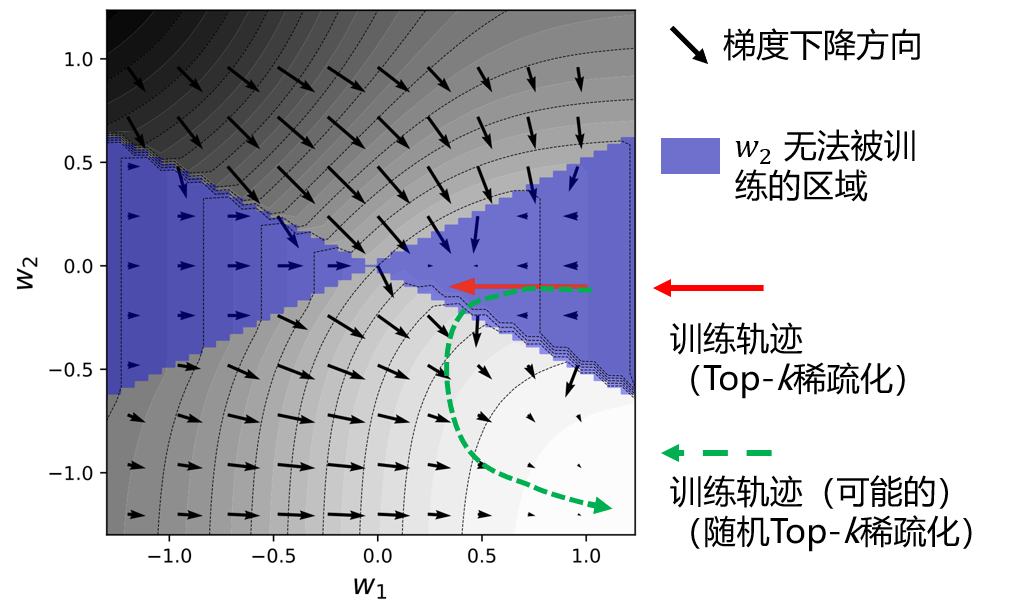
\includegraphics[width=0.75\linewidth]{Z_Resources/randtopk_example.png}
    \caption{使用Top-$k$稀疏化时的损失函数曲面和梯度下降方向}
    \label{fig:randomized_topk:example}
\end{figure}



然而如果在训练过程中使用Top-$k$稀疏化(假设使用平方损失函数),由于$h_2$的值在各个样本上都很小,则$h_2$总是无法被选为Top-$k$,从而导致其对应的权重$w_2$一直无法被训练(对应图中的蓝色区域)。
%
在这种情况下,模型会收敛到一个远离最优点的区域,使得$w_1$降低到$0.4$左右,平衡两个样本的误差,而$w_2$则未被更新而停留在$0.1$处,对应\autoref{fig:randomized_topk:example}中的红色训练轨迹。
%
但是如果在Top-$k$的过程中加入一点随机性,使得$h_2$也有一定的几率被选中,则可以让$w_2$被训练到并且更新,从而摆脱局部最优。
图中的绿色轨迹表明了在Top-$k$稀疏中加入随机性的一条可能的训练轨迹。


Top-$k$稀疏化的收敛问题也会进一步导致其泛化性能降低。
%
如上文所述,Top-$k$稀疏化带来的泛化优势是因为其表征空间包含了$d \choose k$个超球面,其中$d$是原始的拆分层维度(神经元个数),$k$是稀疏化后保留的维度。
%
但是由于Top-$k$稀疏化带来某些神经元(维度)一直难以得到训练的问题,导致某些神经元在各个样本都无法被选中为Top-$k$,从而导致这些神经元被在模型中无法发挥作用,缩小了表征空间的大小。
%
具体而言,如果采用Top-$k$算法进行训练,假设有$d'$个神经元处于“废弃”状态,则最终得到的表征空间中的超球面数目就会从$d \choose k$减少到$d - d' \choose k$。
%
同样地,如果在Top-$k$稀疏化中加入随机性,将使得各个神经元都有一定的机会被训练,提高表征空间的利用率,从而提高泛化效果。


\subsection{随机Top-$k$算法定义}
基于以上分析,我们可以定义如下的随机Top-$k$算法:
%
选择$k$个要保留的神经元时,每一次选择某个神经元的概率为:
\begin{equation}
\label{eq:randomized_topk:def}
    P(\text{选择该神经元}) = 
    \begin{cases}
        (1 - \alpha) / N_1  & \text{如果该神经元是Top-$k$的,} \\
        \alpha / N_2        & \text{反之,}    
    \end{cases}
\end{equation}
%
其中,$N_1$和$N_2$分别表示当前未被选择的Top-$k$神经元数目和非Top-$k$神经元数目。
%
\autoref{fig:randomized_topk:algo}显示了随机Top-$k$算法的可能执行结果。
%
可以看出,$\alpha$表示选择非Top-$k$神经元的概率。
%
当$\alpha=0$时,随机Top-$k$算法退化为普通的Top-$k$稀疏化;而当$\alpha=1$时,则转变为完全随机的Dropout算法~\cite{srivastava_2014_dropout}。
%
注意到,随机Top-$k$仅仅被应用于模型的训练阶段,在推断阶段,我们依然采用确定性的Top-$k$稀疏化。
%
通过实验,我们发现$\alpha \in [0.05, 0.1]$时模型能取得较好的训练效果。
%
\begin{figure}[h!]
    \centering
    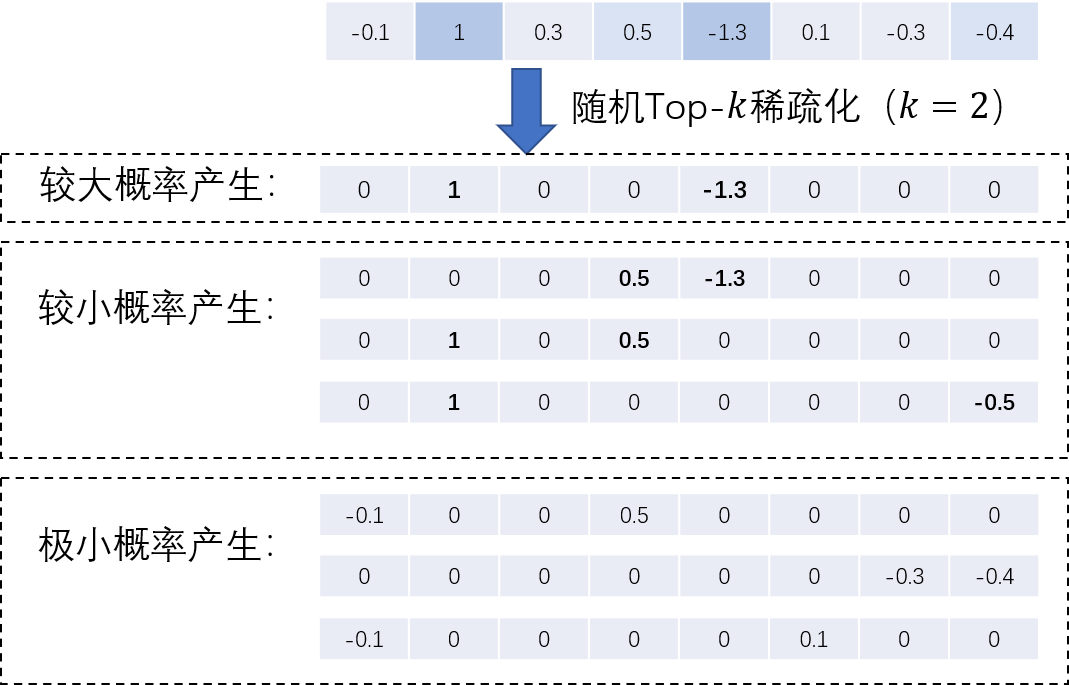
\includegraphics[width=0.7\linewidth]{Z_Resources/randtopk_algorithm.png}
    \caption{随机Top-$k$算法示意图}
    \label{fig:randomized_topk:algo}
\end{figure}


\subsection{隐私分析}
对拆分层表征进行稀疏化后,大部分的拆分层表征元素被丢弃,因此Top-$k$稀疏化或随机Top-$k$稀疏化都能够比原始的拆分学习更多地保护输入特征的隐私。
%
我们在后续实验章节中提供了通过拆分层表征对输入特征进行重建攻击(Reconstruction Attack)的结果。
%
尽管如此,研究表明拆分学习对于标签推理攻击(Label Inference Attack)或模型补全攻击(Model Completion Attack)较为脆弱\cite{fucong2022label_infer_attack},随机Top-$k$算法也并不能解决标签的隐私问题。
%
因此本文考虑的应用场景为标签类别数量大且标签推断攻击不可行的深度学习应用。
%
比如,包含了数千个类别的人脸识别模型、包含了上万种商品的推荐系统模型。
%
对于这些模型,使用者难以获取其他类别对应的输入特征,因此也难以进行标签推断攻击或是模型补全攻击。
%

